\documentclass[hidelinks, 11pt, fleqn]{article}   	% use "amsart" instead of "article" for AMSLaTeX format
\usepackage{geometry}                		% See geometry.pdf to learn the layout options. There are lots.
\usepackage{tikz}
\usepackage{listings}
\usepackage{color}

\definecolor{codegreen}{rgb}{0,0.6,0}
\definecolor{codegray}{rgb}{0.5,0.5,0.5}
\definecolor{lightgray}{rgb}{0.7,0.7,0.7}
\definecolor{codepurple}{rgb}{0.58,0,0.82}
\definecolor{backcolour}{rgb}{0.92,0.92,0.92}

\renewcommand{\lstlistingname}{Algorithm}% Listing -> Algorithm

\lstdefinestyle{mystyle}{
	backgroundcolor=\color{backcolour},   
	commentstyle=\color{codegray},
	keywordstyle=\color{red},
	numberstyle=\tiny\color{lightgray},
	stringstyle=\color{codepurple},
	basicstyle=\footnotesize,
	breakatwhitespace=false,         
	breaklines=true,                 
	captionpos=b,                    
	keepspaces=true,                 
	numbers=left,                    
	numbersep=5pt,                  
	showspaces=false,                
	showstringspaces=false,
	showtabs=false,                  
	tabsize=4
}

\lstset{style=mystyle}

\usepackage{amsmath}
\usepackage{mathtools}
\usepackage{algorithm}
\usepackage{algpseudocode}
\geometry{letterpaper}                   		% ... or a4paper or a5paper or ... 
%\geometry{landscape}                		% Activate for rotated page geometry
%\usepackage[parfill]{parskip}    		% Activate to begin paragraphs with an empty line rather than an indent
\usepackage{graphicx}				% Use pdf, png, jpg, or eps§ with pdflatex; use eps in DVI mode
\usepackage{subcaption}
\usepackage{hyperref}
								% TeX will automatically convert eps --> pdf in pdflatex		
\usepackage{amssymb}

%SetFonts

%SetFonts
\newtagform{brackets}{[}{]}
\usetagform{brackets}

\title{\textbf{Microglider Assembly}}
\author{Patrick Sorn}
%\date{}							% Activate to display a given date or no date

\begin{document}
\maketitle
\tableofcontents 
\pagebreak
\section{Parts}
\subsection{Motor Mount}
Motor Mount (Aluminium):
\begin{figure}[h]
\begin{tikzpicture}
% draw bottom front
\draw[thick] (0,0) -- (0,2) -- (3,2) -- (3,0) -- (0,0);
\draw[dashed] (0,0.2) -- (3,0.2);
\draw (0.5,0.6) circle (1.5mm);
\draw (0.5,1.6) circle (1.5mm);
\draw (2.5,0.6) circle (1.5mm);
\draw (2.5,1.6) circle (1.5mm);
% draw bottom back
\draw[thick] (5,0) -- (5,2) -- (8,2) -- (8,0) -- (5,0);
\draw[thick] (5,0.2) -- (8,0.2);
\draw (5.5,0.6) circle (1.5mm);
\draw (5.5,1.6) circle (1.5mm);
\draw (7.5,0.6) circle (1.5mm);
\draw (7.5,1.6) circle (1.5mm);
% draw front
\draw[thick] (0,5) -- (3,5) -- (3,8) -- (0,8) -- (0,5);
\draw[dashed] (0,5.2) -- (3,5.2);
\draw (0.7,5.7) circle (1.5mm);
\draw (0.7,7.3) circle (1.5mm);
\draw (2.3,7.3) circle (1.5mm);
\draw (2.3,5.7) circle (1.5mm);
\draw (1.5,6.5) circle (8mm);
% draw description
\draw[thick] (0,-0.1) -- (0,-0.5);
\draw[<-] (0.05,-0.3) -- (1.25,-0.3);
\draw (1.5,-0.3) node {$30$};
\draw[->] (1.75,-0.3) -- (2.95,-0.3);
\draw[thick] (3,-0.1) -- (3,-0.5);
% draw back
\draw[thick] (5,5) -- (8,5) -- (8,8) -- (5,8) -- (5,5);
\draw[thick] (5,5.2) -- (8,5.2);
\draw (5.7,5.7) circle (1.5mm);
\draw (5.7,7.3) circle (1.5mm);
\draw (7.3,7.3) circle (1.5mm);
\draw (7.3,5.7) circle (1.5mm);
\draw (6.5,6.5) circle (8mm);
% draw side left
\draw[thick] (10,5) -- (12,5) -- (12,5.2) -- (10.2,5.2) -- (10.2,8) -- (10,8) -- (10,5);
% draw side right
\draw[thick] (14,5) -- (16,5) -- (16,8) -- (15.8,8) -- (15.8,5.2) -- (14,5.2) -- (14,5);
\end{tikzpicture}
\caption{Motor mount front, rear, bottom and side view.}
\label{fig:motor_mount}
\end{figure}
\pagebreak
\subsection{Wings}
The wings are also made out of aluminium.
\begin{figure}[h]
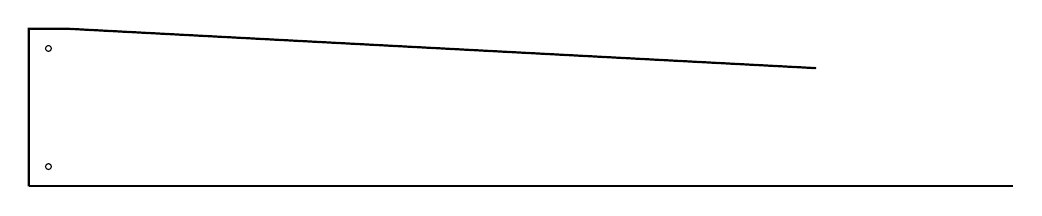
\begin{tikzpicture}
% draw top
\draw[thick] (0,0) -- (0.5,0) -- (12.5,0);
\draw[thick] (10,1.5) -- (0.5,2) -- (0,2) -- (0,0);
\draw (0.25,0.25) circle (0.375mm);
\draw (0.25,1.75) circle (0.375mm);
\end{tikzpicture}
\caption{Wings front, rear, bottom and side view.}
\label{fig:wings}
\end{figure}
\begin{figure}[h]
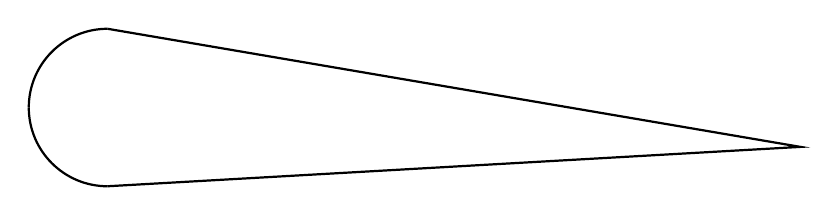
\begin{tikzpicture}
% draw airfoil
\draw[thick] (0.2,3) arc (180:90:10mm);
\draw[thick] (1.2,2) arc (270:180:10mm);
\draw[thick] (1.2,2) -- (10,2.5) -- (1.2,4);
\end{tikzpicture}
\caption{Airfoil of the wing.}
\label{fig:airfoil}
\end{figure}
\end{document}